\documentclass[tikz,border=4pt]{standalone}
\usepackage{tikz}
\usetikzlibrary{arrows.meta,calc}
\begin{document}
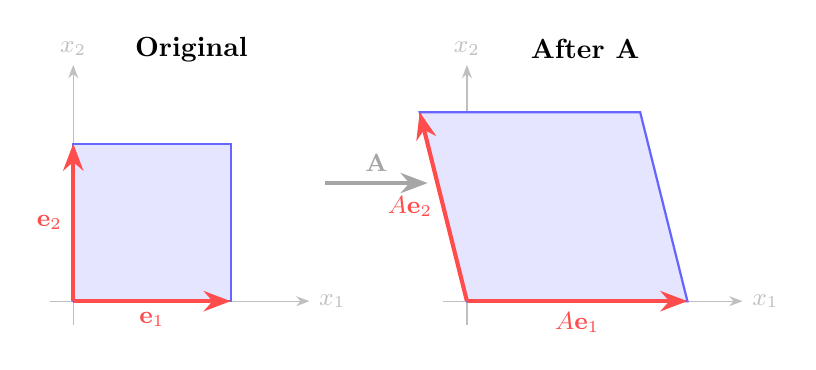
\begin{tikzpicture}[>=Stealth]
    % === Left: original unit square ===
    \begin{scope}
        \node[font=\bfseries] at (1.5,3.2) {Original};
        \draw[->,gray!50] (-0.3,0) -- (3,0) node[right,font=\small] {$x_1$};
        \draw[->,gray!50] (0,-0.3) -- (0,3) node[above,font=\small] {$x_2$};

        % Unit square
        \draw[blue!60,fill=blue!10,thick]
            (0,0) -- (2,0) -- (2,2) -- (0,2) -- cycle;

        % Basis vectors
        \draw[->,red!70,line width=1.5pt] (0,0) -- (2,0)
            node[midway,below,font=\small] {$\mathbf{e}_1$};
        \draw[->,red!70,line width=1.5pt] (0,0) -- (0,2)
            node[midway,left,font=\small] {$\mathbf{e}_2$};
    \end{scope}

    % === Right: after transformation A ===
    \begin{scope}[shift={(5,0)}]
        \node[font=\bfseries] at (1.5,3.2) {After $\mathbf{A}$};
        \draw[->,gray!50] (-0.3,0) -- (3.5,0) node[right,font=\small] {$x_1$};
        \draw[->,gray!50] (0,-0.3) -- (0,3) node[above,font=\small] {$x_2$};

        % Transformed square (shear + scale)
        \draw[blue!60,fill=blue!10,thick]
            (0,0) -- (2.8,0) -- (2.2,2.4) -- (-0.6,2.4) -- cycle;

        % Transformed basis vectors
        \draw[->,red!70,line width=1.5pt] (0,0) -- (2.8,0)
            node[midway,below,font=\small] {$A\mathbf{e}_1$};
        \draw[->,red!70,line width=1.5pt] (0,0) -- (-0.6,2.4)
            node[midway,left,font=\small] {$A\mathbf{e}_2$};
    \end{scope}

    % Arrow between
    \draw[->,line width=1.5pt,gray!70] (3.2,1.5) -- (4.5,1.5)
        node[midway,above,font=\small] {$\mathbf{A}$};
\end{tikzpicture}
\end{document}
